La siguiente figura \ref{fig:System_Architecture} ejemplifica la arquitectura del sistema y de que se compone: \\
% System architecture image
\begin{figure}[hp]
	\centering
	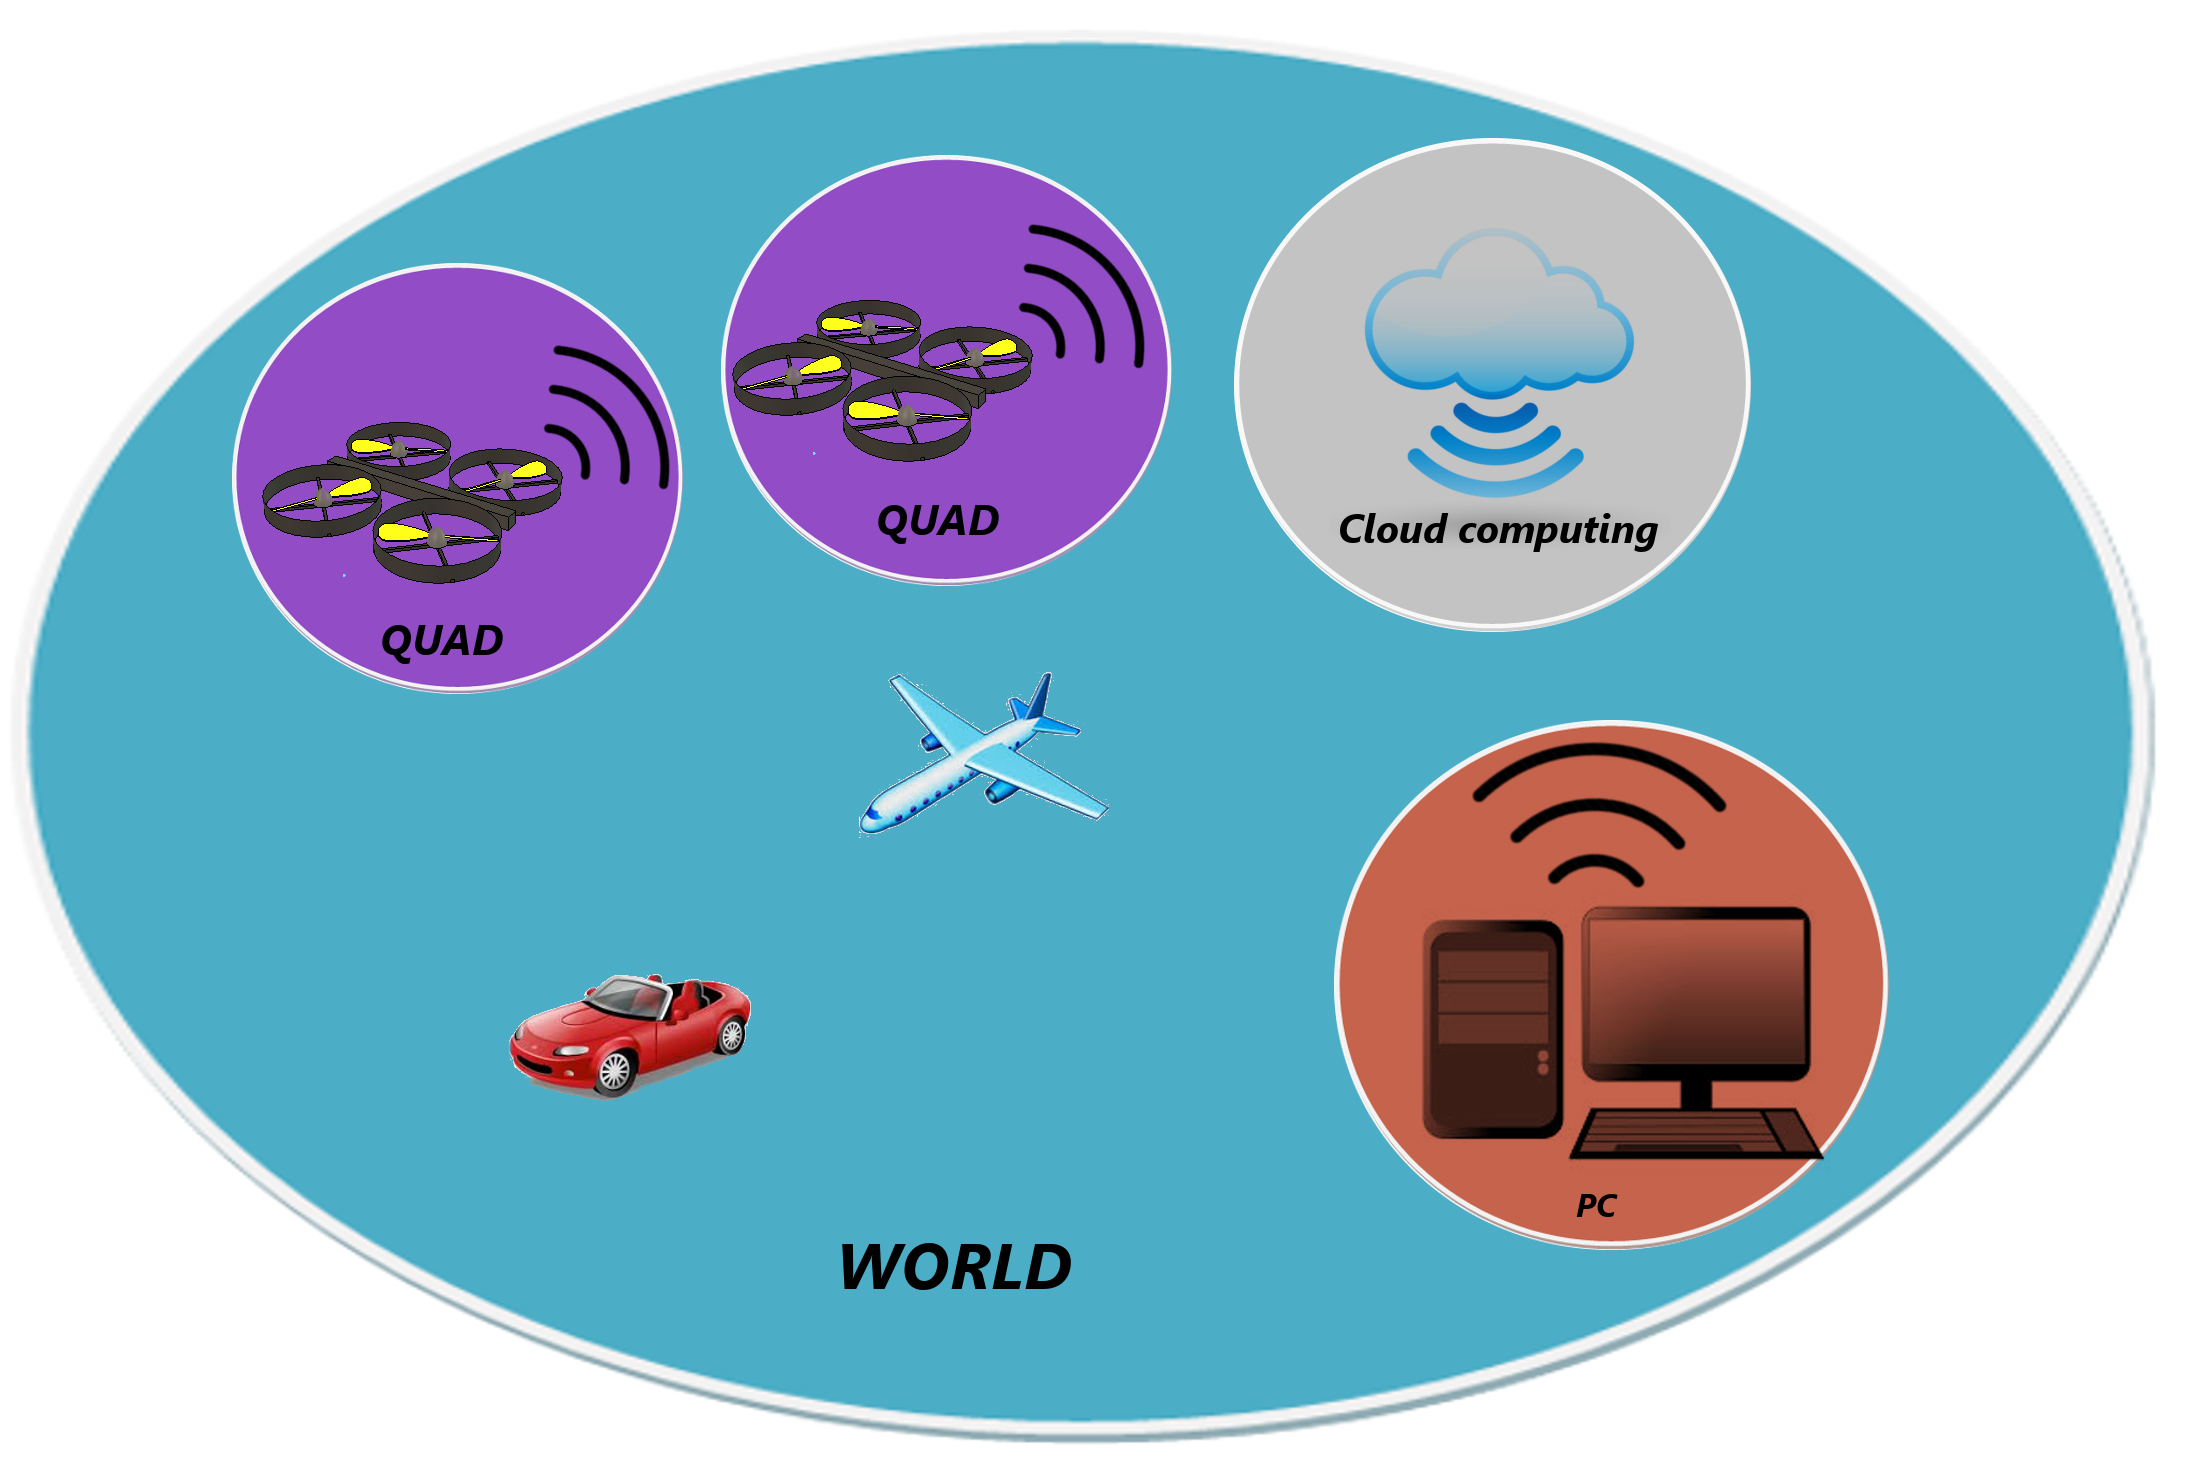
\includegraphics[width=0.50\textwidth,natwidth=220,natheight=1467]{../Images/c2/Architecture.png}
	\caption{Arquitectura del sistema}
	\label{fig:System_Architecture}
\end{figure}


\begin{itemize}
  \item Conjunto de Quadrotores.
  \item Estaci\'on de tierra.
  \item Punto de acceso.
  \item Objetivos.
\end{itemize}

Cada quadrotor consta de una c\'amara y un ordenaddor de abordo que ejecuta el algoritmo, la informaci\'on obtenida se manda a la estaci\'on en tierra que la procesa y ejecuta el algoritmo de seguimiento.

\newpage
\subsection{Quadrotors Software}

	\begin{figure}[hp]
		\begin{center}
			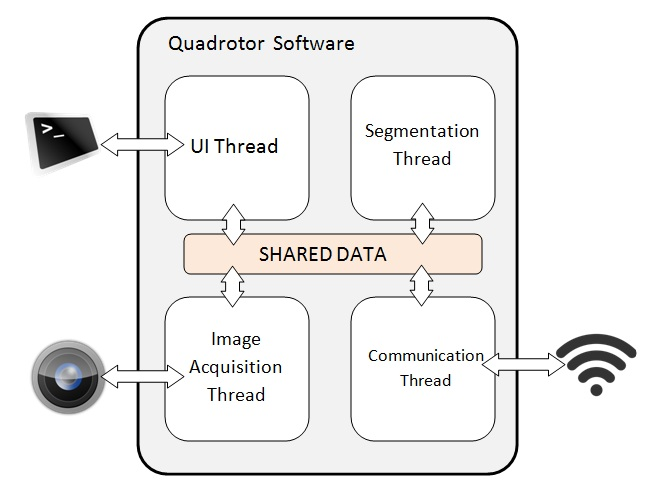
\includegraphics[width=0.7\linewidth]{../Images/c2/Quadsoftware}
		\end{center}
		\caption{Quadrotor's Software}
		\label{fig:Quadsoftware}
	\end{figure}

	La figura \ref{fig:Quadsoftware} muestra esquematicamente la estructura del software de cada quadrotor que se compone de varios threads para paralelizar el algoritmo:
	
	
	\begin{itemize}
		\label{itemize:quadappthreads}
		\item Thread de interfaz de usuario.
		\item Thread de adquisici\'on de im\'agenes.
		\item Thread de segmentaci\'on de im\'agenes.
		\item Thread de comunicaci\'on.
	\end{itemize}
	
\subsection{Software de la estaci\'on de tierra}
	\begin{figure}[th]
		\begin{center}
			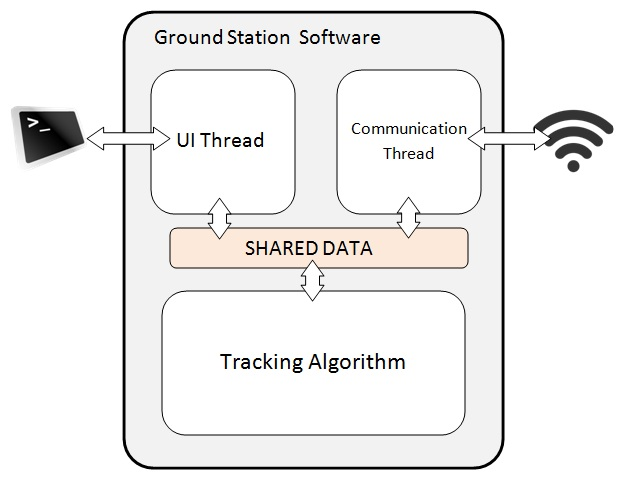
\includegraphics[width=0.7\linewidth]{../Images/c2/GroundStationsoftware}
		\end{center}
		\caption{Ground station's Software}
		\label{fig:GroundStation}
	\end{figure}

	\begin{itemize}
		\item Thread de interfaz de usuario.
		\item Thread de comunicaci\'on.
		\item Thread de algoritmo de seguimiento.
	\end{itemize}

	
\subsection{Conclusion}
La funcionalidad de ambos, quadrotor y estaci\'on de tierra puede ser modificada facilmente añadiendo threads a la ejecuci\'on del programa. Adem\'as gracias a las capas de abstracci\'on cada parte de la estructura puede ser remplazada por otra que la mejore o para adaptar el sistema por ejemplo:

\begin{itemize}
  \item Conjunto de quadrotores $\Longrightarrow$ UGVs y UAVs variados.
  \item Estaci\'on de tierra $\Longrightarrow$ M\'ultiples estaciones de tierra ($Cloud computation$ \cite{Cloud_computing} o estaciones m\'oviles)
  \item Punto de acceso $\Longrightarrow$  M\'odulos GSM ($Cloud computation$ \ref{cloud_computing})
  \item Objetivos.
\end{itemize}


% 666 TODO: terminar